\section{Architecture}
This chapter will describe the architecture of the BF processor in a little more detail, but providing very few implementation details for each of the modules.

\subsection{Overview}
The processor consists of three basic building blocks: registers, memory and a control unit. The ALU is missing from this list because the only operations that it needs to perform is addition and subtraction of the value 1, which can be done directly at the register-level when using up/down binary counters like the 74LS193 integrated circuit. The program (a sequence of BF instructions) is stored into Read Only Memory (ROM), whereas the data is stored in Random Access Memory (RAM). Instructions (4-bits) are loaded from ROM into the instruction register (I), together with some flags that encode the state of the machine. Depending on the state and current instruction, the Control Unit sets the appropriate control signals for each of the modules in order for the system to perform the next computation. Figure \ref{fig:architecture} shows how each of the modules is communicating with other modules. In the sections below, each of these connections will be clarified further.

\begin{figure}[H]
  \centering
  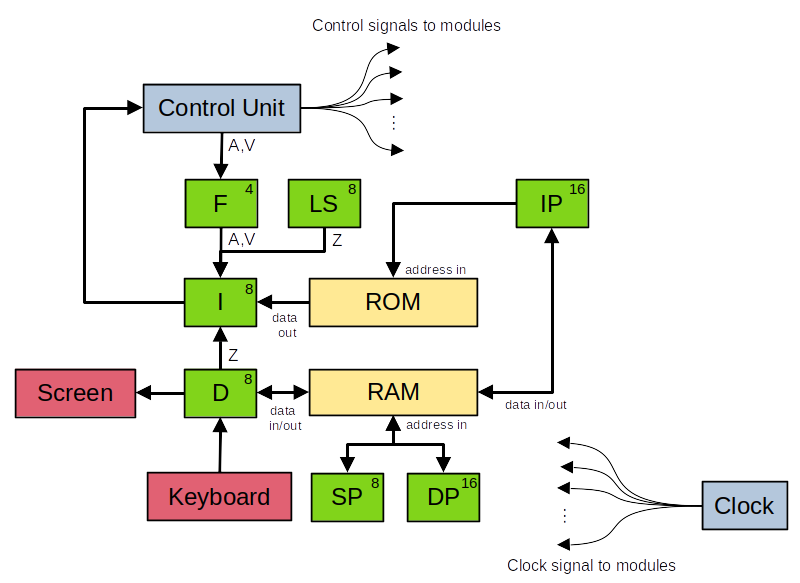
\includegraphics[width=0.9\textwidth]{img/bfcpu_architecture}
  \caption{Connections between modules in the BF processor.}
  \label{fig:architecture}
\end{figure}

\subsection{Instruction Pointer Register (IP)}
The instruction pointer is a 16-bit value, kept in the IP register, which keeps track of the current instruction that is being executed. It points to a certain address in ROM (which stores the program) and is usually incremented after each instruction has finished executing, in order to move to the next instruction. However, when the processor encounters the \texttt{[}-instruction, it needs to store the current value of the IP somewhere: the stack. When the matching \texttt{]}-instruction is encountered, this value is loaded back into the IP instead of simply incrementing the previous value. This has the effect of jumping back in the program, which is how loops are implemented in BF.

\subsection{Stack}
The stack is the first part of RAM (addresses 0x0000 - 0x00ff) which is reserved to keep track of addresses that might need to be jumped to. The stack-pointer (SP) is incremented whenever a new value is stored on the stack and decremented whenever a value is popped off the stack. In this implementation, the SP is an 8-bit value, which means that at most 256 different values can be stored onto the stack before it starts leaking into data-memory (stack overflow). This would happen if a BF program was loaded that has more than 256 nested \texttt{[]}-pairs. Although possible, it is very unlikely to happen for the simple programs we intend to run.

\subsection{Instruction Register}
The instruction register is an 8-bit register that stores the current instruction, which was loaded from ROM according to the IP value. The BF-instruction itself is only 4 bits wide, which leaves another 4 bits for encoding the state of the machine, using flags. There are 4 flags that determine the state of the machine:
\begin{itemize}
\item Z(D): the zero-flag set by the D-register, indicating that there is currently a 0 stored in this register;
\item Z(LS): the zero-flag set by the LS-register (see below);
\item A: the address-changed-flag, set by the control-unit, indicating that the previous instruction has changed the value of the data-pointer. When this flag is set, the value in the D-register does no longer correspond to the cell pointed to by the data-pointer;
\item V: the value-changed-flag, set by the control-unit, indicating that the previous instruction has altered the value in the D-register. When this flag is set, the value in RAM is outdated and needs to be updated before moving the pointer to a different cell.
\end{itemize}

\subsection{Data Register (D) and Data Pointer Register (DP)}
The data-pointer corresponds to the pointer as specified in the BF-language. It points to some value in memory and can be either incremented (\texttt{>}) or decremented (\texttt{<}). Whenever a value is modified by \texttt{+} or \texttt{-}, this value has to be loaded into the D-register, where it can be modified before being stored back into RAM.


